% <- percent signs are used to comment
\documentclass[12pt]{article}

%amsmath is a packaged use for typesetting math
%amsfonts is required f	or special fonts, e.g. blackboard bold (for denoting real numbers, etc.)
\usepackage{amsmath,amsfonts}

%graphicx is required for images
\usepackage{graphicx}

%used for customzing enumarations
\usepackage{enumerate}

%tikz is the package used for trees
\usepackage{tikz}

\usepackage{algo,fullpage,url,amssymb,epsfig,color,xspace}
\usepackage[pdftitle={Final Report},%
pdfsubject={University of Waterloo, SE 350, Winter 2016},%
pdfauthor={}]{hyperref}
\usepackage{titlesec}

\setcounter{secnumdepth}{4}

\titleformat{\paragraph}
{\normalfont\normalsize\bfseries}{\theparagraph}{1em}{}
\titlespacing*{\paragraph}
{0pt}{3.25ex plus 1ex minus .2ex}{1.5ex plus .2ex}

\renewcommand{\contentsname}{Table of Contents}

%Note: Many of the packages above have other uses beyond those used in this document

%this marks the beginning of the document. Everything before this is called the Preamble.
\begin{document}
%marks the end of the title section
\begin{center}
{\Large\bf University of Waterloo}\\
\vspace{3mm}
{\Large\bf SE350, Winter 2016}\\
\vspace{80mm}
{\Large\bf RTX Project Final Report}\\
\vspace{80mm}
\textbf{Chen Pin Jie, 20516440, pjchen} \\
\textbf{Rahman Md Wasiur, 20511250, mwrahman} \\
\textbf{Duncan Philip Oudom, 20527971,  poduncan} \\
\textbf{Hariharan Ajanthan, 20526424, a2hariha} \\

\end{center}

\definecolor{care}{rgb}{0,0,0}
\def\question#1{\item[\bf #1.]}
\def\part#1{\item[\bf #1)]}
\newcommand{\pc}[1]{\mbox{\textbf{#1}}} % pseudocode

\clearpage
\tableofcontents
\newpage
\section{Introduction}
This report is about Group 6’s design and implementation of the real-time executive (RTX). The operating system was implemented on a Keil MCB1700 board populated with an NXP LPC1768 microcontroller. The operating system provides a basic multiprogramming environment, with five priority levels, preemption, simple memory management, message-based inter-process communication, a basic timing service, system console I/O and debugging support.\\ \\
The purpose of this report is to provide the readers an overview of the design of the operating system. This report will give the readers the knowledge to effectively use the operating system. \\ \\
The first section of the report contains the list of all the important global variables that was used in the implementation of the operating system. The second section of the report contains the documentation of the kernel APIs. The third section of the report will cover all the interrupts and their handlers/processes. The fourth section of the report will describe the all the system and user processes. The fifth section of the report will explain in detail what happens at OS bootup. The sixth section of the report will provide the details on the testing and debugging techniques we used as part of the development of the operating system. This section will also contain the timing analysis of some of the functions. The final part of the report contain major design changes and lessons we learned from the development of the operating system.
\newpage
\section{Global Variable Documentation}
\textbf{gp\_currentpcb} - This variable is the process control block of the current running process. This variable is important because we can use it to determine and change the current running process.\\ \\
\textbf{gp\_pcbs} - This variable is an array of the all the process control blocks. The PCBs are indexed by their process ids. This variable is important because we can use it to easily access and change processes\\ \\
\textbf{g\_proc\_table,  g\_test\_procs, g\_sys\_procs, g\_i\_procs} - These variables are used to initialize the processes.\\ \\
\textbf{g\_switch\_flag} - This is a global flag that determines whether to continue to run the process before the UART receive interrupt. If g\_switch\_flag == 0, then restore the process that was interrupted. Otherwise (i.e g\_switch\_flag == 1), then switch to the other process.\\ \\
\textbf{priority\_q}  - This is a linked list of PCBs. There are 4 priority\_qs, one for each priority. This is used by scheduler to determine which process to execute next. When process change priority, they are moved to a different priority\_q.\\ \\
\textbf{g\_timer\_count} - This is an integer that maintains the milliseconds count of the overall system. It is used for two reasons. Firstly, every time this counter increments, we assign g\_second\_timer = g\_timer\_count / 1000. Secondly, we use this timer as a reference to determine when a delayed message should be sent. \\ \\
\textbf{g\_second\_count} - This is an integer that maintains the seconds count for the wall clock. Another variable is used to keep track of the seconds since the wall clock can set the seconds count to zero as well as any other value. If we used the g\_timer\_count to keep track of the seconds, modifications to the wall clock would have been impossible since changing the value of g\_timer\_count will result in unexpected behaviours in delayed messaging.\\ \\
\textbf{command\_head} - This is a linked list data structure. It is used to keep track of the commands that have been registered with the KCD as well as the process that registered the commands. It is a global variable because during initialization, the predetermined commands such as \%WT and \%WS are manually inserted into this structure. Therefore, we need a reference to this from the system initialization process and the KCD process. \\ \\
\textbf{terminated} - This is an integer that is either 1 or 0. If it’s 1, then the wall clock process is terminated. Otherwise, the wall clock process is set to running and the update\_clock method sends updated time messages to the CRT process. This is a global variable because reference to this is made from update\_clock and KCD process. 
\section{Kernel API}
\subsection{Memory Management}
Memory blocks can be used by user process in order to make make arrays and other data structures. The memory management API consists of two public methods, request\_memory\_block() and release\_memory\_block(). In memory\_init().\\ \\
Memory blocks are implemented a pointer to a memory address. All free memory blocks are contained in a linked list, where the start of the linked list is stored in free\_mem. The memory management APIs use this linked list to retrieve and release memory blocks.
\subsubsection{Request Memory}
\begin{verbatim}
                        void * request_memory_block() 
\end{verbatim}
The request\_memory\_block function is called when a user process requires a memory block. The function takes in zero parameters and returns a pointer to the start of the memory block. \\ \\
If the free\_mem does not point to null, and there are available memory block, a memory block is removed from the linked list, free\_mem is updated and the pointer to the memory block is returned. When the free\_mem points to null, there are no more available memory blocks to return. In this case the calling process is blocked and release\_processor is called until there is an available memory block. 
\subsubsection{Release Memory}
\begin{verbatim}
                int k_release_memory_block(void *p_mem_blk)
\end{verbatim}
The release\_memory\_block function is called when a user process is finished with their requested memory block. The function takes in a pointer to the memory block that the user wants to release and return an int that shows whether or not the release was successful. If memory block was successfully released the function would return 0, otherwise if an error occured the function would return -1. \\ \\
When a memory address is passed in, the memory address is verified to be a valid memory block. If the memory block is invalid an error code of -1 returned. If the memory block is valid and free\_mem is null, there can be a process that is blocked on memory. The memory block is added into the linked list, and all memory blocked processes are checked to see if preemption is necessary. If preemption is necessary then release\_processor is called and the function is released with an error\_code of 0. 
\subsection{Process Management}
\subsubsection{Release Processor}
\begin{verbatim}
                        int release_processor()
\end{verbatim}
The process that calls release\_processor will release the the processor to the RTX. release\_processor is called when the current process is finished executing, or if the current process wants to voluntarily release the processor to another process. This function also called when the current process is blocked or pre-empted. release\_processor() takes no input parameters and returns 0 if the function completes with no error. If the there are no processes it can switch to it will return -1 and return the control of the processor to the invoking process. \\ \\
When the function is invoked the invoking process’ state will be changed from running to ready and is put at the end of the ready queue of the same priority. If there exist other processes in the ready queue of the same or higher priority then they will be selected for execution. If there are no other ready process of higher or same priority then the invoking process will be at the front of the ready queue and it will be selected for execution. The process that will be selected for execution will change its state to running and set the stack pointer to the current process’ PCB.
\subsubsection{Set Process Priority}
\begin{verbatim}
          int set_process_priority(int process_id, int priority)
\end{verbatim}
set\_process\_priority() allows the invoking process to change the priority of any process (including the invoking process). set\_process\_priority() takes two parameters process\_id and priority, and the function returns an integer. This function will return 0 if the function completes with no error. If the process\_id does not belong to any user or system process or if the priority is not between 0 and 3 then the function will not change any priorities and return 1.\\ \\
When the function is invoked the PCB with same pid as the process\_id (first input parameter) will have its priority set to priority (first input parameter). Then the PCB will be dequeued from ready queue of its old priority and enqueued into the end of the read queue of its new priority. If the old priority and the new priority are the same then the PCB will simply be moved to the end of the queue. The function then calls p\_findAllproc, which return the process with the highest priority and that is also ready. If the process returned by p\_findAllproc is the current process then function will finish and return 0. If the process returned is another process then the current process will call release\_processor(), which will allow the higher priority process to preempt the current process.
\subsubsection{Get Process Priority}
\begin{verbatim}
                int get_process_priority(int process_id)
\end{verbatim}
get\_process\_priority returns the priority of the PCB specified by the process\_id parameter. If the id is invalid, get\_process\_priority will throw an exception.
\subsection{Interprocess Communication}
\subsubsection{Send Message}
\begin{verbatim}
      int k_send_message_i(int process_id, void * message_envelope)
\end{verbatim}
This functions takes in the receiver process\_id, message object pointer. The sender process indicated what process the caller would like to send the message to and returns an error code. The message pointer is a user constructed msgbuf object that contains the message they would like the send and the message type. In order to construct the message, the user process will have to request and use a memory block. \\ \\
The function will set the m\_recv\_pid and the m\_sender\_pid of the message\_envelope. The message\_envelope is then added to the receiver's message queue. If the receiver process is currently message blocked, the process will be set to ready. If the receiver process has a higher priority than the current process preemption will take place. If the function executed till completion, the function will return 0, informing the user process that the message was successfully sent. 
\subsubsection{Receive Message}
\begin{verbatim}
                 void* k_receive_message(int * sender_id)
\end{verbatim}
This function takes in the sender\_id pointer and return a msgbuf object pointer. If the current process’s message queue is not empty, the first message is returned and the sender\_id pointer is set the process id of the functions that sent the message. If there are no messages in the message queue of current process, the current process is messaged blocked and release processor is called. 
\subsubsection{Delay Send Message}
\begin{verbatim}
    int delayed_send(int process_id, void * message_envelope, int delay)
\end{verbatim}
delayed\_send() allows processes to send messages that will not be received until a time delay has passed. This is implemented by sending the message to the Timer i-process for temporary storage. The Timer i-process eventually sends the message to the specified recipient after the delay has passed, using the message’s m\_expiry property. delayed\_send() sets m\_expiry before sending the message to the Timer i-process by adding the delay argument to the current system time.\\ \\
As an edge case, if delay is 0, delayed\_send() simply calls send\_message() since no delay is necessary. An exit status 1 occurs if the the specified recipient process\_id argument is not a valid PID.
\section{Interrupts and their Handlers/Processes}
\subsection{Timer I-Process}
The timer i-process is called every time the hardware issues a timer interrupt. It handles the delivery of delayed messages. It operates as follows. \\ \\
\begin{verbatim}
TIMER0_IRQHandler {
    save context
    timer_i_process()
    branch to POP_STACK if no preemption flag
    release_processor()
POP_STACK
    return context
}

timer_i_process {
    for each message in mailbox:
        add message to priority queue
    while message in priority queue expired:
        send message to recipient
        if the recipient is message_blocked and has higher priority:
            set preemption flag
}s
\end{verbatim}
\subsection{UART I-Process}
This process is responsible for inputted characters from UART0 and outputting. Before the IRQ is run the IRQ\_handler saves the state of all the current registers. After the IRQ is handled the registers are restored and if preemption is necessary, then release\_processor() is called, otherwise the interrupted process is restored.   \\ \\
For an inputted character, after the interrupt is disabled, the inputted character is added into an input buffer. When the carriage return “\textbackslash r” or a new line “\textbackslash n” is inputted the current input buffer content is sent to KCD, and the buffer is cleared. The KCD will then be responsible to dealing with the message and sending the message to CRT to print the message. \\ \\
The UARI-Process can have its interrupt bit set by KCD, indicating that a message is needed to be printed on the console. The message is received, and output buffer is set to the message’s content. The UART-IProcess cannot be message blocked because if the UART is interrupted for a message to output by the CRT, a valid message must also be sent. The output buffer is outputted onto the console, the output\_buffer is reset and the interrupt is cleared. \\ \\
UARTI-Process operates as follows: \\ \\
\begin{verbatim}
UARTI_PROC(){
   if (data is inputted into the console) { 
		clear the interrupt
		if(g_char_in =='\n'||g_char_in =='\r'){
			add a null character to the buffer
			send the contents of the buffer to KCD
			clear_buffer()
		}else{
			g_buffer[g_buffer_index] = g_char_in;
			g_buffer_index++;
		}	
		#ifdef _DEBUG_HOTKEYS
		//hot key interrupts
		if ( g_char_in == 'q' || g_char_in =='w' || g_char_in=='e' ) {
			print hotkey message
		}
		#endif
	} else if (data need to be outputted into console) {
		if(!is_message_empty(UART_PROC_ID)){
			message = k_receive_message(&sender_id);
			gp_current_process=orig_proc;
			if(message!=NULL){
				gp_buffer=message->mtext;
				output gp_buffer
				reset gp_buffer
				g_switch_flag = k_release_memory_block_i(message);
			} 
}
	}
}
\end{verbatim}
\subsubsection{Debugging Hotkeys}
The debugging hotkey are used to make debugging problems with our OS easier. The hot keats ‘q’, ‘w’, ‘e’ print out the ready processes, memory blocked process and message blocked process respectively. The the hot keys are pressed a list process id’s with their corresponding priority are printed. These hotkeys will be enabled when the operating system is compiled with the \_DEBUG\_HOTKEYS flag enabled.

\section{System and User Processes}
\subsection{System Processes}
\subsubsection{Null Process}
The Null process is the only process that has the lowest priority 4. This is so that it only runs when no other process is running. It is implemented as an infinite loop of calling release\_processor(). This is effectively checking if there is some other process of higher priority to switch to. If such a process exists in the system, context is switched away from the Null process so that the other processes can run.
\subsubsection{KCD Process}
The KCD process is in charge of registering and delegating keyboard commands to appropriate processes. It keeps track of all registered commands and the process associated with those commands. It also allows the registration of commands shorter than 10 characters. A command is denoted with the ‘\%’ symbol, followed by the command alias, followed by a terminating space character. \\ \\
The KCD handles two types of messages. The first type of message it handles is of type ‘Default’. Default messages have the potential to contain special commands. The KCD is in charge of parsing the message body to detect the existence of such commands. The commands that the KCD is looking for have already been registered and is stored in a linked list. When the KCD detects messages starting with the ‘\%’ character, it takes the word following that character and searches the linked list. If the command exists, the message is wrapped in a message envelope and sent to the process associated with that command. If the command is not found in the linked list, then no action is performed. For instance, if the linked list contains the command ‘X’ and is associated with ‘handle\_x’ process, then a message starting with ‘\%X …’ will be detected by the KCD process. The KCD process will then proceed to wrap this message body in a new message envelope and send it to the process ‘handle\_x’. Note, the KCD process releases the message sent by the process since it simply packs it another envelope when sending it to the associated process.\\ \\
The KCD also handles messages of type ‘KCD\_REG’. This type of message indicates that there is a command that needs to be registered and added to the linked list maintained by the KCD. The KCD process takes the command and adds it to the list. It also creates an association between this new command and the process that sent the message. In the future, during the decoding stage, if a message is found with the following command, it will be sent to the process that registered this command. After the registration, the KCD process releases the message.
\subsubsection{Clock Process}
The clock process handles three commands: \%WR, \%WS, \%WT. The time format that the clock process abides by is HH:MM:SS. Any time specified by the user conforms to this format. During startup, the clock process registers the specified commands with the KCD. Therefore, the KCD will forward those messages to the clock process. Once the message is received, the clock process still has to distinguish between the three commands. The process reads the first two characters following the ‘\%’ to determine how to process the message. Any message that does not begin with those keywords (which should not be forwarded to the process to begin with) will be ignored. \\ \\
The clock process maintains a global variable that tracks the number of seconds elapsed since the clock has been reset and running. It also maintains a global flag called ‘terminated’ which is set to true if the clock is not running. There is already a system variable that maintains a milliseconds count. This variable is leveraged to keep track of the seconds count. When we detect the second count has increased and the terminated variable is set to false, the seconds variable is increased and the updated time is sent to the CRT process from the timer.c’s update\_clock method. \\ \\
During the incrementing stage, there is an edge case that needs to be accounted for. When the clock reaches 23:59:59, the clock should loop around to 00:00:00. To allow for this to take place, the hour value is modded by 24. Therefore, it never goes above 24 hours.\\ \\
When the clock process detects the \%WR command, it will reset the wall clock. To reset the clock, we simply set the global seconds count variable to 0. In addition to resetting the clock, it also starts the clock if the clock had previously been stopped. The global ‘terminated’ flag gets set to true after this command is processed. \\ \\
When the clock process detects the \%WS command, it verifies whether the rest of the message conforms to the HH:MM:SS (hours:minutes:seconds) format. If the message does not follow this format, it sets the clock to 00:00:00. If the message is valid, then we take each of the values for hour, minutes and seconds and convert it to a seconds value. Then we set the global seconds variable to the value of the new calculated seconds. Finally, the terminated flag is set to false to allow the clock to run. \\ \\
Finally, the wall clock process also detects the \%WT command. This command simply sets the global terminated variable to true. This results in the update\_clock method in the timer.c code to not send the updated time to the CRT process. Thus, the clock stops updating.
\subsubsection{CRT Process}
The CRT process is responsible for delegating text output to the terminal. In order for a process to output to the terminal, it sends a message containing that text to the CRT process.\\ \\
When the CRT process receives a message of type CRT\_DISPLAY, it outputs its containing text to the terminal via the UART i-process. It does so by passing on the message to the UART i-process and setting the relevant IER flag in the LPC\_UART0 hardware. This triggers a UART0\_IRQ interrupt so the UART i-process starts.
\subsubsection{Set Priority Process}
The set priority process is a process to change the priority of a running process to a new priority. When the system is initialized, the command \%C is registered with the KCD process by the set\_priority\_process. This ensures that all keyboard input starting with \%C is sent to this process for handling. \\ \\
The set priority process accepts messages of the format ‘\%C [process id] [new priority]’. The process id ranges from 1 to 13 and does not allow the NULL process and the interrupt process to be changed since they have fixed priorities. \\
New priority excludes the priority value of 4 since it's the lowest priority and is reserved for the NULL process.\\ \\
Upon receiving a message from the KCD, it does validation on the process id and new priority value to ensure that the above properties hold. If the command is valid, we call the set\_process\_priority(process id, priority) method to change the priority of the specified process.
\subsection{User Processes}
\subsubsection{User Test Process}
6 user processes were created to test the functionalities of the APIs. Here are the list of the functionalities that were tested by the user process.\\ \\ 
\textbf{set\_priority, get\_priority} - This is tested by setting all the user process to priority 3. Test process 1 will be executed because it was inserted first into the priority queue during initialization. Test process 1 then sets the priority of process 3 to 1 by calling set\_process\_priority(3, 1); . Then test process 3 check if it pre-empted process 1, since test process 3 now has a higher priority. Test process 3 then calls get\_process\_priority(3) to check if its priority is correctly set to 1. \\ \\
\textbf{request\_memory\_block,  release\_memory\_block} - This is tested by having test process 3 request all the memory blocks. Test process 3 then checks if the last block it requested has the same address as the address of the last block. Then set the priority of process 2 to highest so process 2 is executed. Test process 2 will then try to call request\_memory\_block. This will block test process 2 because test process 3 requested all the memory blocks. The control of the processor should then return to test process 3. Then process 3 checks if test process 2’s state is BLK using the gp\_pcbs global variable. Then process 3 will release a memory block and process 2 will check if it’s unblocked. \\ \\
\textbf{send\_message,  receive\_message }- This is tested by having test process 1 call send\_message(2, env). Then process 1 releases processor to process 2. Process 2 then calls receive\_message() and check if the content of the message is the same as the message sent by process 1. Process 2 then calls receive\_message() again which message blocks process 2 and returns the control back to process 1. Process 1 then calls send\_message(2, env2) and check if process 2 is unblocked.\\ \\
\textbf{delayed\_send} - This is tested by having test process 3 call delayed\_send(2, env2, 10). Then process 3 set priority of process 2 to a higher priority which allows process 2 to pre-empt process 3. Process 2 then calls receive\_message() immediately which will message block process 2 since the message have not arrived yet. The control of the processor will then return to process 3. Process 3 will execute for 10 seconds until process 2 receives the delayed message and becomes unblocked and pre-empts process 3. Process 2 then checks the content of the message to make sure it is correct.
\subsubsection{Stress Test Process}
\textbf{Stress Test A}\\ \\
Stress Test A start off by registering the command with KCD by sending a message with “\%Z”, with type reg\_kcd to KCD. This process then goes into a loop that calls recieve\_message, which will message block itself. When the user types in “\%Z ” into the console, the message will be set to stress test A and the second loop will be called.\\ \\
The second loop will constantly call request\_memory\_block() and which is used to create message. The message is set to have type COUNT\_REPORT, and is sent to stress test B. The process will eventually use up all the memory and memory block itself.\\ \\
\textbf{Stress Test B}\\ \\ 
Stress Test B constantly receives messages from Stress test A and send the messages to stress Test C. When Stress Test B tries to receive a message when there are no messages, it message blocks itself. \\ \\
\textbf{Stress Test C}\\ \\ 
Stress Test C makes a buffer queue called msg\_q that holds all the inputted messages. First test C checks if msg\_q is empty. If it is empty then recieve\_message() is called, message blocking the process until a message is received. If msq\_q is not empty a message is popped from the queue and is processed. \\ \\
If the received message is not of type COUNT\_REPORT, then the memory block used from the received message is released.  If the received message is of type COUNT\_REPORT, then the m\_kdata field of the message is received. The received value is modded by 20 is 0, then a message type is set to CRT\_DISPLAY, the contents of the message is set “Process C” and is sent to CRT process. If the received value modded with 20 is 1, then a delayed message is sent to stress test B with type WAKEUP10 and a delay of 10 seconds. Once this occurs a inner loop is entered and test C is ‘hibernating’. \\ \\
In the inner loop, test C calls receive\_message() and message blocks itself. When it receives a message it checks if the message is of type WAKEUP10. If the message type is WAKEUP10 test C stops ‘hibernating’, exits the inner for-loop, releases the memory of message and continues to pop messages from the msg\_q. If the message is not of type WAKEUP10, then the message is received and added to the msg\_q in order to be read later. 
\newpage
\section{Initialization}
\subsection*{Timer Initialization}
This initializes the hardware for timer interrupts. The Prescale Register is set to 12499, which makes the Timer Counter toggle between 0 and 1 every 12500 PCLKs. After also setting MR0, setting MCR, enabling TCR, and calling NVIC\_EnableIRQ(), this results in a 1 mHz Counter. An internal second counters and a release flag are initialized to 0 to set the initial state of the Timer i-process. As final result, the hardware triggers a branch to the TIMER0\_IRQHandler label every millisecond.
\subsection*{UART Initialization}
This initializes the hardware for keyboard interrupts (specifically the RBR, THRE or RX lines). This is done by configuring the Pin Control Block and transmission standards (to line up with the standards set in the PuTTY terminal). The buffer is set to trigger 1 character per interrupt on a first-in-first-out basis. As a final result, the hardware triggers a branch to the UART0\_IRQHandler label for every keystroke, and every time a process sets the THRE bit.
\subsection*{Memory Initialization}
Space is made available between RAM\_TOP and Image\$\$RW\_IRAM1\$\$ZI\$\$Limit for the heap, PCBs, and stacks. The space made available for stacks is calculated based on the number of processes and the predetermined size of a stack. The heap is initialized with a set number of fixed-sized memory blocks which are linked together in a linked list. Space for PCBs is initialized similar to the stacks, where the number of processes made available and the set size of a PCB is factored in.
\subsection*{Process Initialization}
The user processes, system processes, stress processes, and interrupt-driven processes are all initialized. In each case, the PCBs which were allocated in Memory Initialization are used to store information about each process, including process ID, initial process priority, and stack size.
\newpage
\section{Testing}
The functionality of the operating system was tested with unit testing, regression testing, and integration testing. Each person implemented different parts of the operating system and each person is responsible for unit testing the features that they implemented. We created unit tests for every function and data structure we created. When performing unit testing, we use white box testing to ensure that no error occurs. This allows us to easily isolate bugs and potential problems. After we thoroughly tested the individual parts we implemented, we integrate the parts and perform integration testing on the entire system. Integration testing allows us to find bugs that were introduced when integrating different parts of the operating system. Lastly, we perform regression testing after the every major change. This is to make sure the new changes did not break any of the features that we implemented previously. We use the black box testing for integration and regression testing to ensure that our program produced the correct output with a given input. \\ \\
We tested our operating system both manually and automatically. We created automated tests to test features such as our API functions. The automated tests calls different functions and prints different debug statements depending on the result of the call. For certain things such as KCD, CRT and hotkeys we performed manual testing. During manual testing we manually type the inputs and compare the actual output with the expected output.
\subsection{Debugging}
We used the debugger extensively for finding and fixing bugs. We used the watch feature of the debugger to monitor the different objects and global variables. The watch feature allows us to see not only the content of variables but also the memory address of variable. We also used the step through feature of the debugger to identify hard faults. To identify the specific line that caused the hard fault, we step over the lines of code prior to the hard fault until we reach the line that causes the program to hard fault.
\subsection{Timing Analysis}
For the timing analysis, we needed another timer for the measurements since the measures are in the order of microseconds. The original timer is not sensitive enough for this. To implement another timer, we the new timer’s TCR register to 1. To get the time value, we simply get the value of the TC register in the timer. \\ \\
To measure the times, the experiment was run 30 times and the average value was taken. 
\subsubsection{send message}
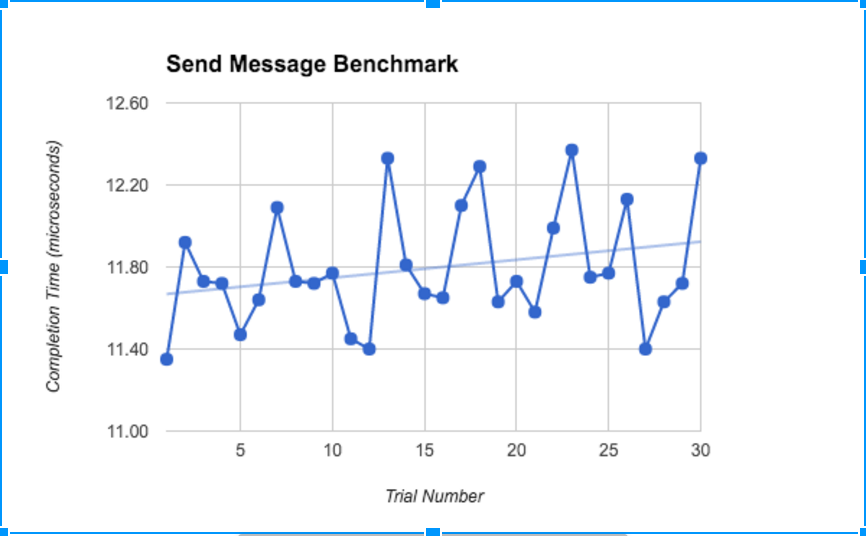
\includegraphics[scale=1]{pic1.png} 
\subsubsection{receive message}
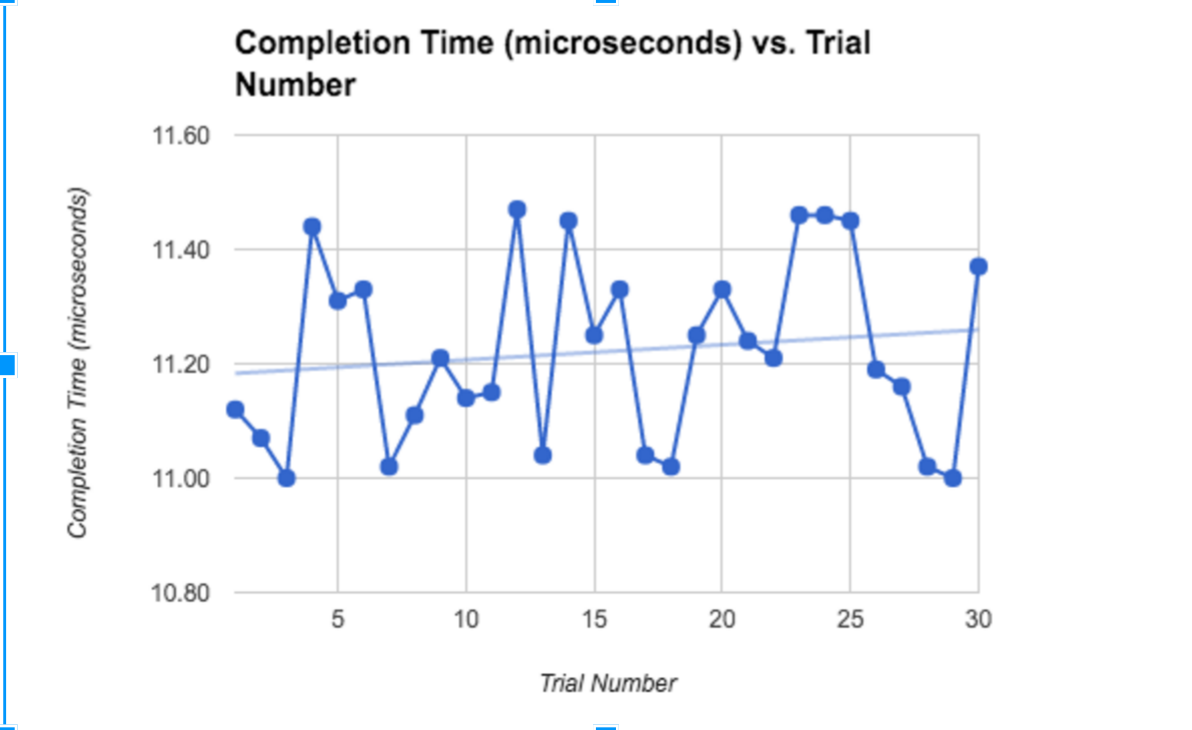
\includegraphics[scale=0.8]{pic2.png} 
\subsubsection{request memory block}
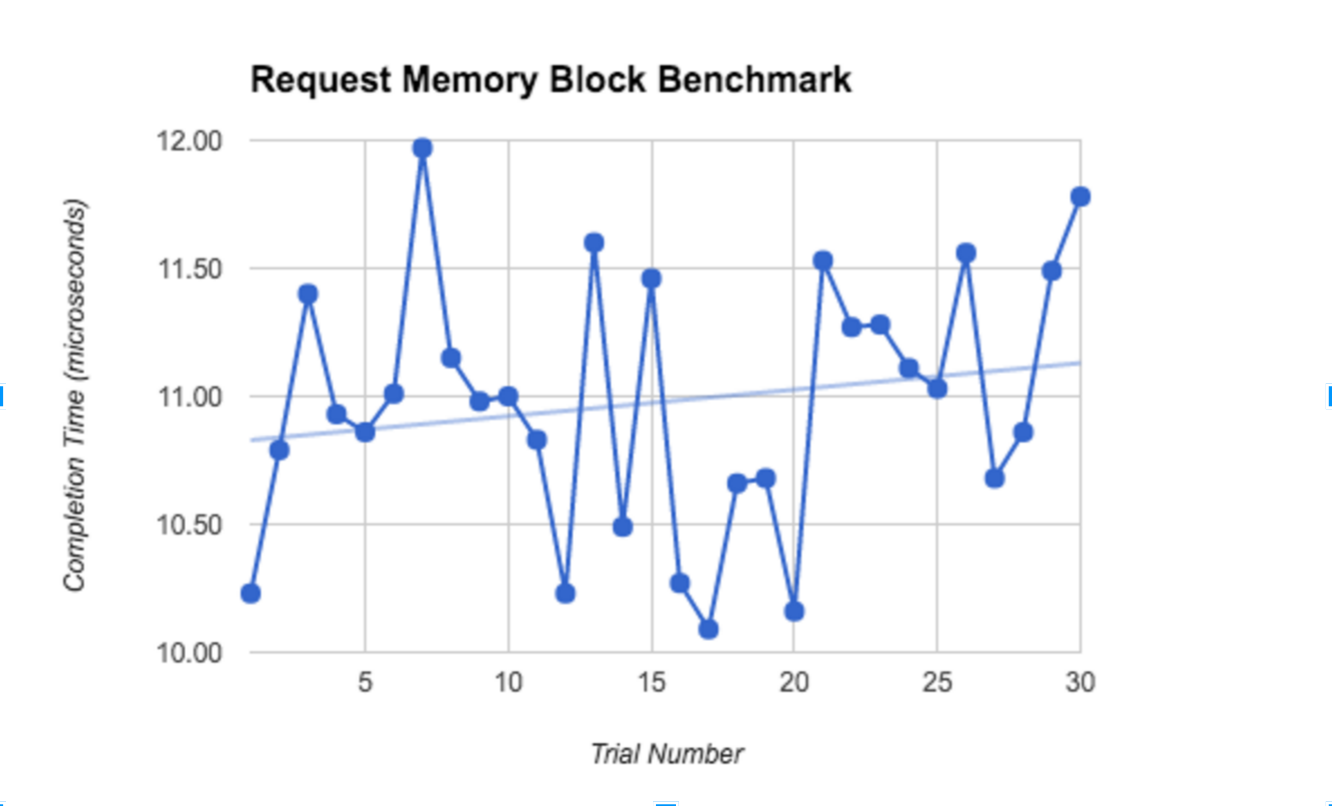
\includegraphics[scale=0.7]{pic3.png} 
\newpage
\section{Major Design Changes}
One of the problems that we initially ran into was hard-faults when commands were inputted into the console when the OS was being run on the board. These hard-fault would occur when the user typed into the console while the timer process was printing out its times every second. The cause for this hard fault was later found be due to the use of a single buffer for both input and output nodes. When testing on the simulator since timer interrupts fired approximately 40 times slower than on the board, the buffer would never have input and output characters inputted into the buffer at once. This was fixed by refactoring the UARTI-Process to have two buffers, one for input and one for output. \\ \\
One of the design changes was to not have seperate queues for message blocked, memory blocked and ready processes. Instead all processes were placed inside the four priority queues. This design decision allowed us to easily change the state of the  processes without having to to dequeue or enqueue the processes. However, our implementation makes it ineffeicient to print out all the processes of a certain state because we have to iterate through all the processes and check their state.\\ \\
One of our design changes was to not the process ids outlined in the lab manual. We instead assigned process ids to our system processes based on the order of implementation. This turned out to be a huge mistake. Due the different process ids that we used, our operating system would not work when using object code provided by the TAs. To solve this problem we created a array that maps our process ids to the correct process ids. \\ \\
\section{Lessons learned}
Many of our coding problems can be rooted at our limited understanding when we began coding. There were a lot of contrived architecture choices as a result of combining together some of the example code. In many cases, we spent a large portion of time writing code from scratch when there was sample code available for the task we were implementing. We could have also saved time by asking more questions during lab sessions. In later sessions, we worked better since we each had a better understanding of the end-goals and we were able to divide up work effectively.\\ \\
During the development of the operating system, there were many occasions where our code worked on the simulator but not on the board. We spent a lot of time debugging the cause of these problems. If we were to start over, we would develop our operating system without the simulator to avoid the compatibility issues.\\ \\
We faced another problem while writing documentation. A lot of undocumented code needed to be reviewed, some of which had not been worked on for months. It would be better in the future to document more while code is being written.
\end{document}